\documentclass[a4paper, 12pt]{article}


\title{Integrated fault detection in distributed decision-making}

\usepackage[english]{babel}

\usepackage[left=1.5cm, right=1.5cm, top=2.5cm, bottom=2.5cm]{geometry}
\usepackage{hyperref}


\usepackage{caption}
\usepackage[labelformat=simple]{subcaption}
\renewcommand\thesubfigure{(\alph{subfigure})}
\usepackage[toc, page]{appendix}
\usepackage{bm}

\usepackage{graphicx}
\graphicspath{{image/}}

\usepackage{amsmath, amsfonts, amssymb}
\usepackage{xspace}

\usepackage{amsthm}
\usepackage{cleveref}
\theoremstyle{plain}
\newtheorem{theorem}{Theorem}
\newtheorem{assumption}[theorem]{Assumption}
\newtheorem{definition}[theorem]{Definition}
\newtheorem{axiom}[theorem]{Axiom}
\newtheorem{lemma}[theorem]{Lemma}
\newtheorem{example}[theorem]{Example}

\newcommand{\argmin}{\operatornamewithlimits{arg\,min}}
\newcommand*{\eg}{e.g.\@\xspace}
\newcommand*{\ie}{i.e.\@\xspace}

\makeatletter
\newcommand*{\etc}{%
    \@ifnextchar{.}%
        {etc}%
        {etc.\@\xspace}%
}

\usepackage{float}

\usepackage{listings}


\begin{document}
\section{Installation on Window}
\subsection*{Miniforge}
First, install \href{https://github.com/conda-forge/miniforge}{Miniforge3} for Windows x86 64.\\
	
\noindent
Open Miniforge Prompt, it is slightly different from Windows' Terminal

\begin{figure}[H]
  \centering
  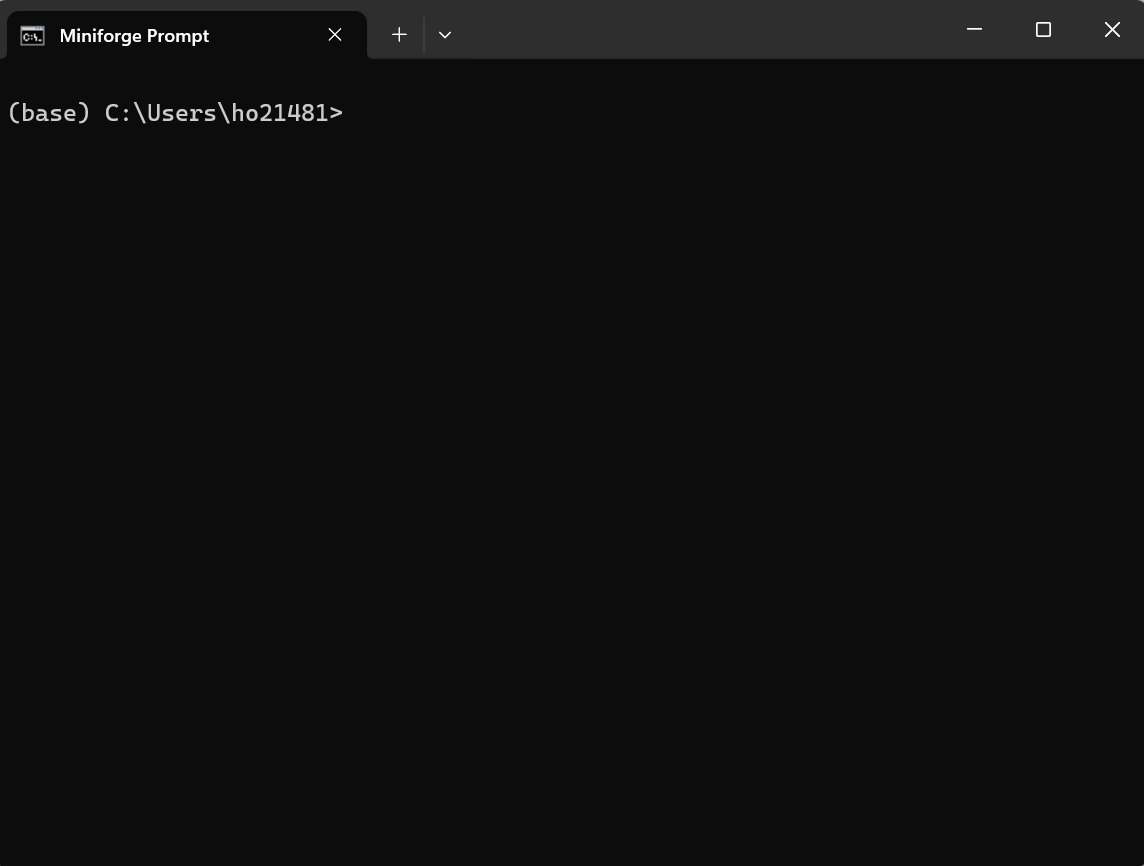
\includegraphics[width=0.7\textwidth]{Prompt}
  \caption{Miniforge Prompt}
\end{figure}


\subsection*{Salvus}

(base) means you are in the virtually environment named base. And then you need to download the list of Python dependencies:\\
\begin{lstlisting}[language=bash]
$ curl https://mondaic.com/environment-py311.yml -o environment.yml
\end{lstlisting}
\vspace{1cm}

\noindent
and create a new virtual environment named salvus with the Python dependencies installed in the file environment.yml:\\

\begin{lstlisting}[language=bash]
$ mamba env create -n salvus -f environment.yml
\end{lstlisting}
\vspace{1cm}

\noindent
Then activate the virtual environment salvus:

\begin{lstlisting}[language=bash]
$ conda activate salvus
\end{lstlisting}
\vspace{1cm}


\begin{figure}[H]
  \centering
  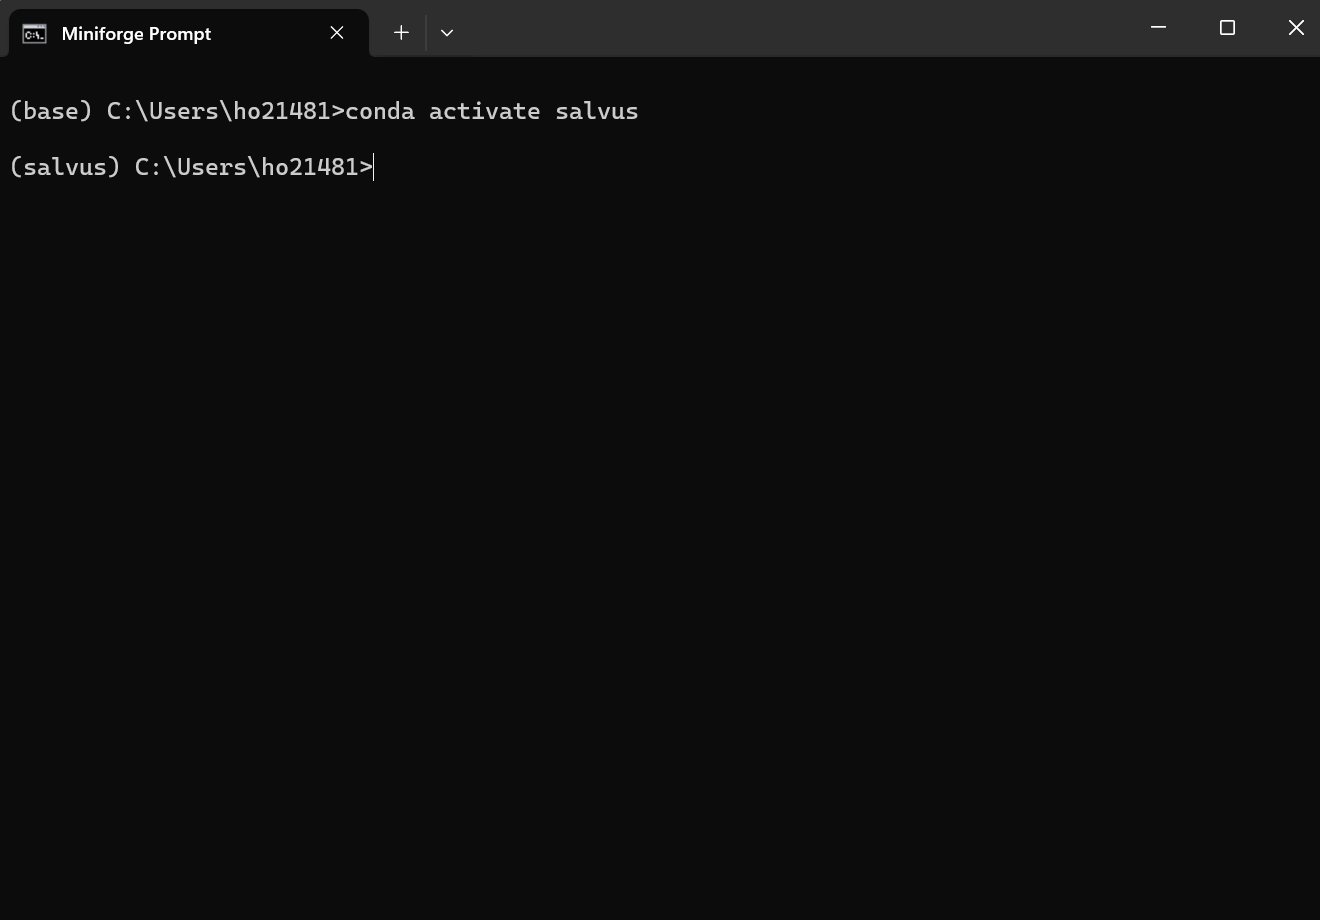
\includegraphics[width=0.7\textwidth]{activate_salvus}
  \caption{Activate the virtual environment named salvus}
\end{figure}

(salvus) indicates that you are in the virtual environment named salvus.\\

\noindent
To download Salvus and install the Salvus Python module, first run the Mondaic Downloader: \\

\noindent
\$  \hspace{0.1cm} powershell -command "iex (New-Object System.Net.WebClient).DownloadString('https://get.mond\\aic.com/win')" \\



\noindent
Enter the following license information prompted as shown in \Cref{fig:Download}.\\
 
\noindent
license username: \textbf{bristol.support} \\
Password: \textbf{scah-bamp-POMP-vair}\\

\begin{figure}[H]
  \centering
  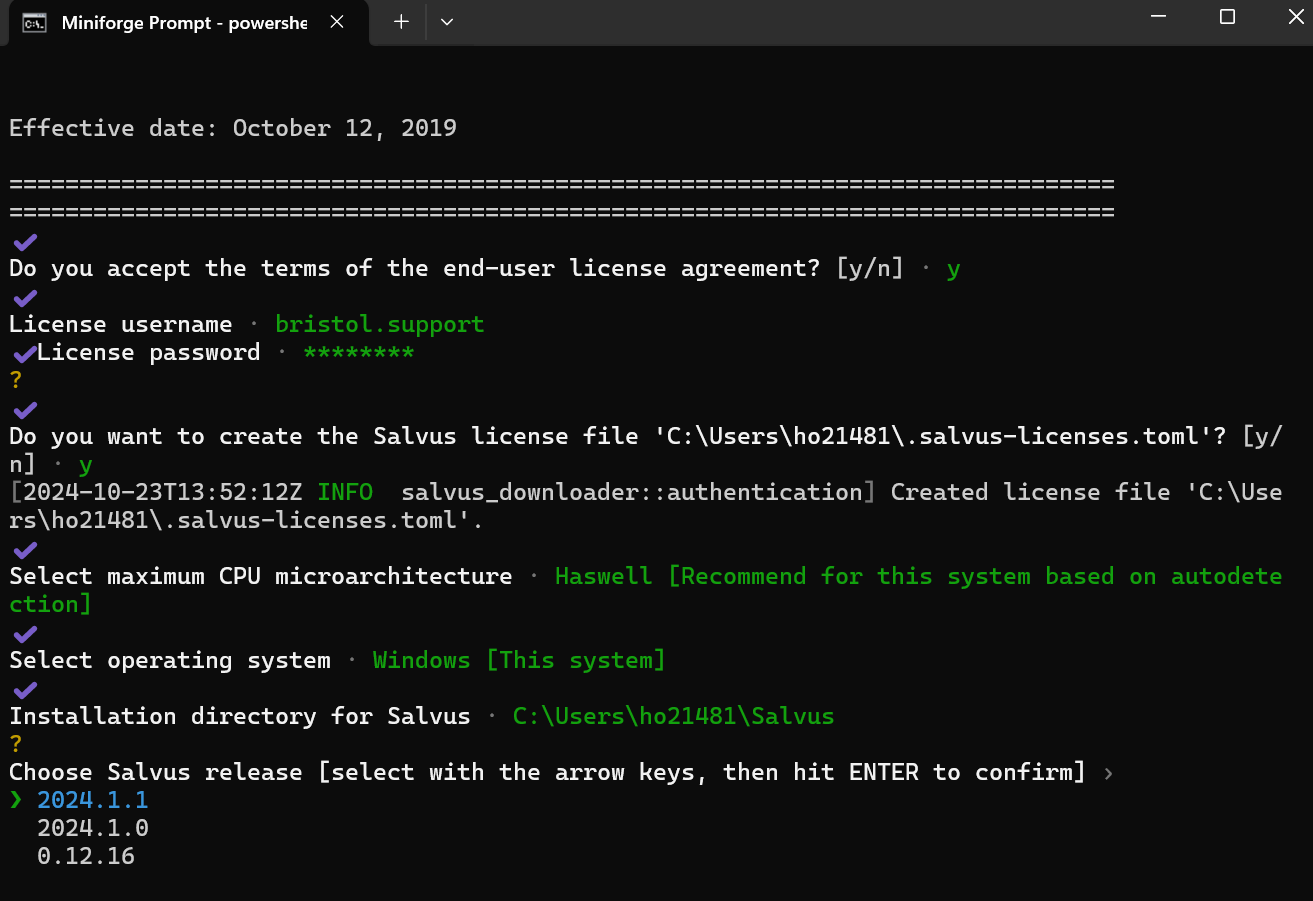
\includegraphics[width=0.7\textwidth]{downloader}
  \caption{Download Salvus}
    \label{fig:Download}
\end{figure}

\noindent
Always choose recommended options and finally it shows in the \Cref{fig:final}

\begin{figure}[H]
  \centering
  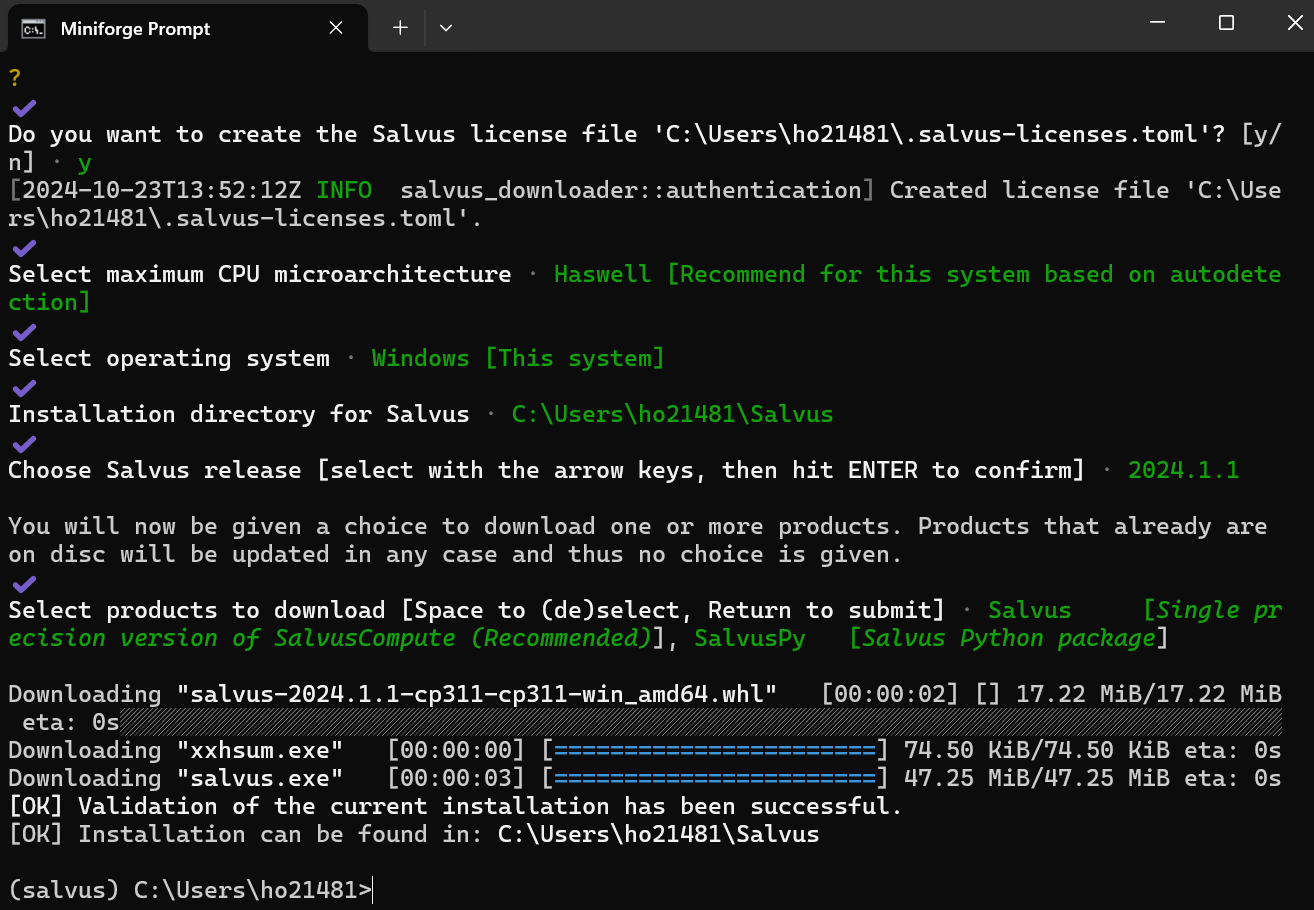
\includegraphics[width=0.7\textwidth]{final}
  \caption{Download Salvus}
  \label{fig:final}
\end{figure}

\noindent
And then install the Salvus Python package with: \\

\begin{lstlisting}[language=bash]
$ cd Salvus\python_packages
$ pip install salvus-2024.1.1-cp311-cp311-win_amd64.whl 
\end{lstlisting}
\vspace{1cm}

make sure you are in the correct directory and the *.whl file exists in the current directory.

\subsection*{Configure SalvusFlow}
The last step is to teach Salvus how to run on your specific machine. Please run this interactive wizard to get started as shown in \Cref{fig:config}, ensure that you are in the virtual environment named salvus otherwise enter commend: \$ conda activate salvus.\\

\begin{lstlisting}[language=bash]
$ salvus-cli add-site
\end{lstlisting}
\vspace{1cm}

\begin{figure}[H]
  \centering
  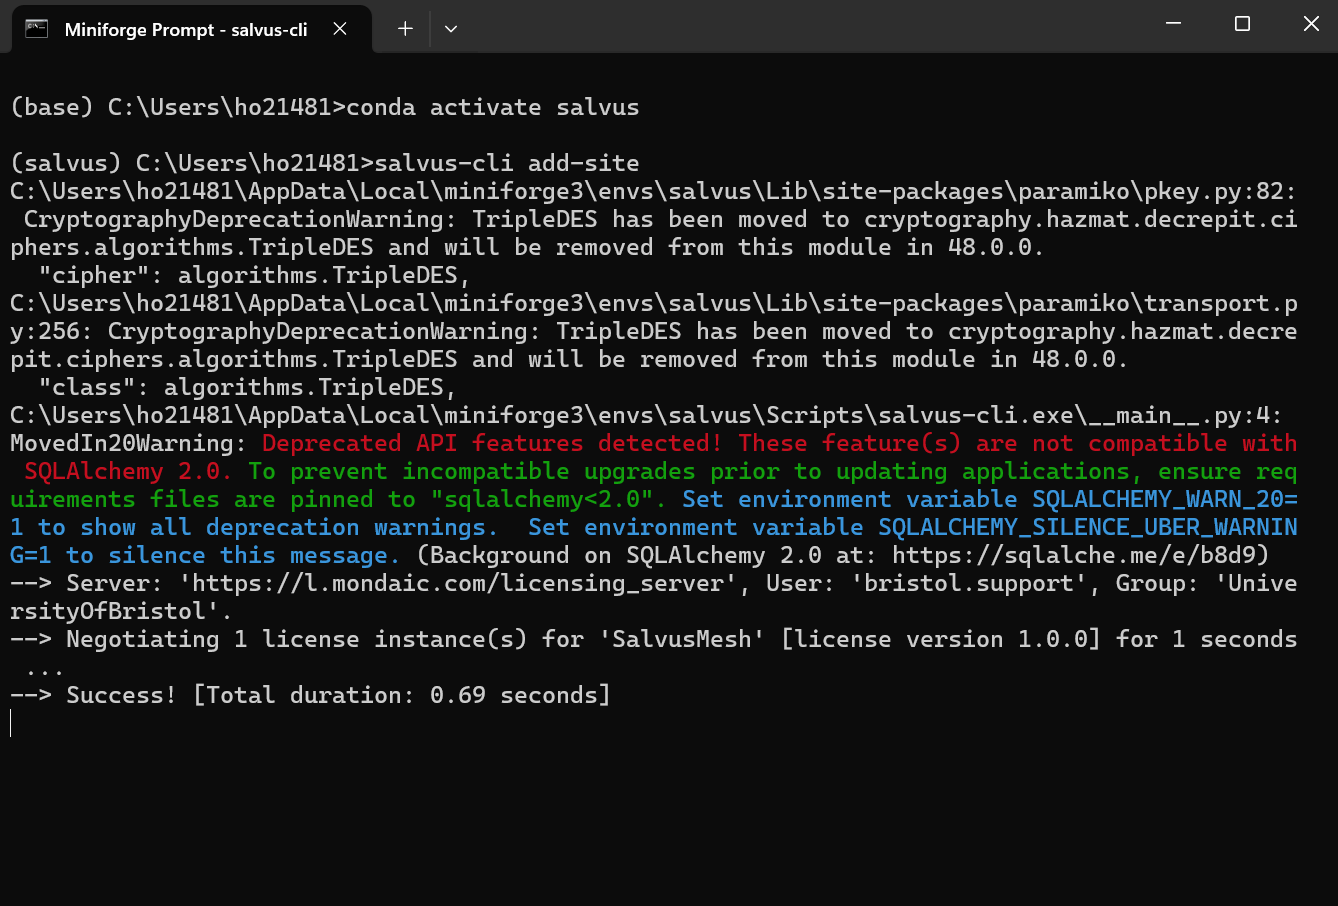
\includegraphics[width=0.7\textwidth]{config}
  \caption{Download Salvus}
  \label{fig:config}
\end{figure}

\noindent
Select "Already installed" for the question "Do you want to install Salvus on remote machine or is it installed?" as shown in \Cref{fig:config_detail}, and always enter "y" or choose default options for the others.

\begin{figure}[H]
  \centering
  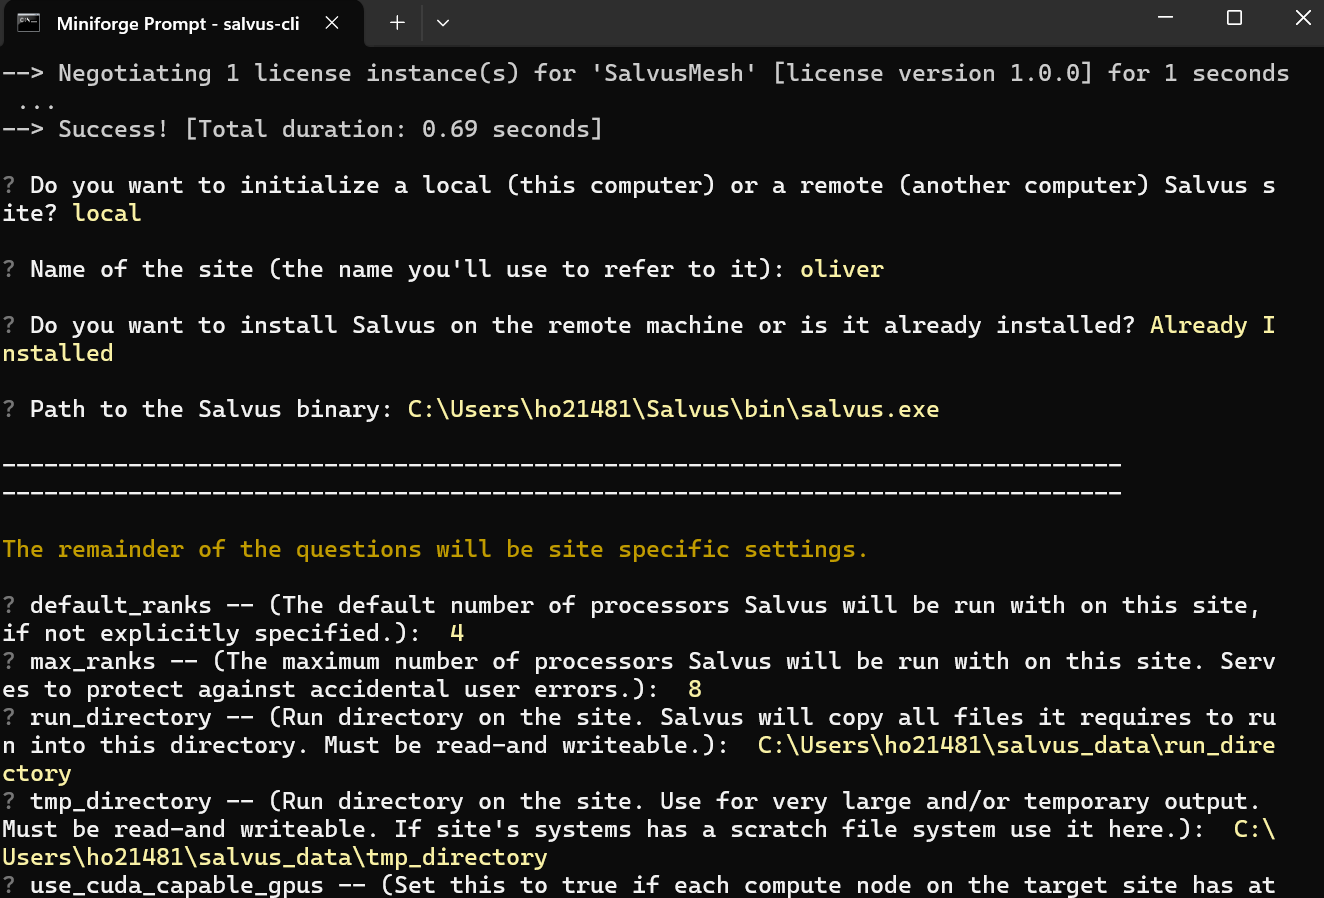
\includegraphics[width=0.7\textwidth]{config_detail}
  \caption{Download Salvus}
  \label{fig:config_detail}
\end{figure}



\newpage

\section{Installation on Linux or MacOS}
\subsection*{Miniforge}

First, install \href{https://github.com/conda-forge/miniforge}{Miniforge3} by running the command below in your terminal:\\

\noindent
\$  \hspace{0.1cm} curl -L -O "https://github.com/conda-forge/miniforge/releases/latest/download/Miniforge3-\$(un\\ame)-\$(uname -m).sh"
bash Miniforge3-\$(uname)-\$(uname -m).sh\\



\subsection*{Salvus}
Then you need to download the list of Python dependencies:\\

\noindent
\$  \hspace{0.1cm}mamba env create -n salvus -f environment.yml\\
\noindent
\$  \hspace{0.1cm}conda activate salvus\\

\noindent
To download Salvus and install the Salvus Python module, first run the Mondaic Downloader: \\

\noindent
\$  \hspace{0.1cm}bash -c "\$(curl -sSL https://get.mondaic.com)"\\

\noindent
Enter the following license information as it requires.\\
 
\noindent
license username: \textbf{bristol.support} \\
Password: \textbf{scah-bamp-POMP-vair}\\

\noindent
And then install the Salvus Python package with:



\noindent
%\$  \hspace{0.1cm}pip install ~/Salvus/python_packages/salvus-*.whl


\begin{verbatim}
$ pip install ~/Salvus/python_packages/salvus-*.whl
\end{verbatim}

\subsection*{Configure SalvusFlow}

The last step is to teach Salvus how to run on your specific machine.\\	


\begin{lstlisting}[language=bash]
$ salvus-cli add-site
\end{lstlisting}
\vspace{1cm}
Select "Already installed" for the question "Do you want to install Salvus on remote machine or is it installed?", and always enter "y" or choose default options for the others.




\end{document}